% !TEX root = ./main.tex
\section{Empirical Bacterial Growth Laws}
\label{sec:emp_laws}

In recent years, there has been a tremendous advancement in our understanding
bacterial physiology from a theoretical perspective. The group of
Terrence Hwa has proposed and tested a series of empirical ``growth laws'' based on experimental observations of cellular behavior \cite{Scott2010,Deris2013}. A major observation is the law that describes a linear relationship between the fraction of the proteome dedicated to ribosomes and growth rate of the cell,
\begin{equation}
    \lambda = (r_u - r_\mathrm{min})\kappa_t\label{equ:growthlaw1},
\end{equation}
where $\lambda$ is the growth rate, $r_u$ is the proteomic fraction of active ribosomes, $r_\mathrm{min}$ is the minimal fraction of ribosomes needed for growth and $\kappa_t$ is an empirically determined proportionality factor called translational capacity. Another result of their study was that the observed cells responded to translation inhibiting drugs by increasing the ribosome fraction of the proteome. Surprisingly, this relationship was also found to be linear,
\begin{equation}
    \lambda = (r_\mathrm{max} - r_\RM{tot}) b\label{equ:growthlaw2}
\end{equation}
In the absence of drug, these two equations are equal to each other, and $r_\RM{tot} = r_u$. We can use this to determine the proportionality factor $b$,
\begin{eqnarray}
    b&=&\frac{1}{\lambda_0}(r_\RM{max}-r_u) \nonumber\\
    &=&\frac{1}{\lambda_0}\left(r_\RM{max}-\frac{\lambda_0}{\kappa_t}-r_\RM{min}\right)\nonumber \\
    &=&\frac{\Delta r}{\lambda_0} - \frac{1}{\kappa_t},
\end{eqnarray}
where we inserted equation \ref{equ:growthlaw1} for $r_u$. Now we can solve for the total ribosomes $r_\RM{tot}$,
\begin{eqnarray}
    r_\RM{tot} &=& r_\RM{max} - b\lambda \nonumber\\
    &=&r_\RM{max} - \lambda \left(\frac{\Delta r}{\lambda_0} - \frac{1}{\kappa_t}\right) \nonumber\\
    &=& r_\RM{max} - \Delta r\lambda \left( \frac{1}{\lambda_0} - \frac{1}{\kappa_t\Delta r} \right)\label{equ:rtot}.
\end{eqnarray}


\section{Derivation of Drug Inhibition}
\label{sec:drug_inhib}
Tetracycline binds the small subunit of the ribosome and stalls translation by inhibiting tRNA from binding \textcolor{purple}{(citation)}. It can be assumed that the drug enters the cell via passive diffusion \textcolor{purple}{(citation)} with flux $J_\RM{in}$,
\begin{equation}
    J_\RM{in} = P_\RM{in} a_\RM{ex} - P_\RM{out} a,
\end{equation}
where $a_\RM{ex}$ is the extracellular concentration of drug, $a$ is the intracellular drug concentration and $j$ is a proportionality constant. In our model, cells gain resistance by expressing drug specific secondary efflux pumps (antiporter), which draw energy from a chemical gradient. In the case of the tetracycline antiporter, the drug is exported against a protein gradient. We assume that the proton gradient is constant for the duration of the experiment (\purple{something we could think about more in detail later}). In this case, the drug kinetics can be described by a Michaelis-Menten equation describing a flux $J_\RM{ex}$
\begin{equation}
J_\RM{ex} = V_\RM{max} {a \over a+K_M},
\end{equation}
where $K_M$ is the Michaelis constant of the efflux pump and $V_\RM{max}$ is the maximum efflux rate which depends on the expression of the resistance gene. In this model we include growth mediated feedback to gene expression \cite{Deris2013}. That is, if growth rate is reduced, so is the expression of genes in the cell (\purple{is this obvious or do we need to prove, e.g. which Heinemann data}),
\begin{equation}
V_\RM{max} = {\lambda\over\lambda_0} V_0,
\end{equation}
where $V_0$ and $\lambda_0$ are the catalytic rate and growth rate in the absence of drug. A detailed dissection of $V_0$ and how it depends on regulation of the resistance gene is given in section \ref{sec:gene_expression}.\\
Tetracycline binds reversibly to the ribosome, therefore we can describe the binding kinetics with
\begin{equation}
    f(r_u, r_b, a) = -k_\RM{on}a\,(r_u-r_\RM{min}) + k_\RM{off} r_b,
\end{equation}
where $k_\RM{on}$ is the binding rate of drug to free ribosome, $k_\RM{off}$ is the dissociation rate of the drug-ribosome complex, and $r_b$ is the concentration of bound ribosomes. In the binding term, we consider the difference of free ribosome to minimum ribosome concentration needed for growth, the model is based on the empirical growth laws, which are not defined for $r_u < r_\RM{min}$.
Using these terms, we can write down the ODE's describing the concentration of drug and ribosomes,
\begin{eqnarray}
    {d a\over d t} &=& -\lambda a + f(r_u, r_b, a) + J(a_\RM{ex}, a) - V_0 {\lambda\over\lambda_0}{a\over a + K_M},\label{equ:dta}\\
    {dr_u\over dt} &=& -\lambda r_u + f(r_u, r_b, a) + s(\lambda),\label{equ:dtru}\\
    {dr_b\over dt} &=& -\lambda r_b - f(r_u, r_b, a)\label{equ:dtrb},
\end{eqnarray}
where $s(\lambda)$ is the rate at which new ribosomes are synthesized. Here we are looking for steady state solutions to find a relationship between growth rate and extracellular drug concentration.
To start, we solve the first empirical growth law \ref{equ:growthlaw1}  for the concentration of free ribosomes, $r_u = \lambda/\kappa_t + r_\RM{min}$ and use it to find the concentration of bound ribosomes by solving equation \ref{equ:dtrb}
\begin{eqnarray}
    0 &=& -\lambda r_b + k_\RM{on}a\,(r_u-r_\RM{min}) - k_\RM{off} r_b \nonumber\\
    &=& -\lambda r_b + k_\RM{on}a\frac{\lambda}{\kappa_t} - k_\RM{off} r_b \nonumber\\
    \Rightarrow r_b &=& k_\RM{on}a{\lambda/\kappa_t \over \lambda + k_\RM{off} } \approx {k_\RM{on} a\lambda \over k_\RM{off} \kappa_t}={a\lambda \over K_d \kappa_t},
\end{eqnarray}
where we simplified $k_\RM{off} + \lambda \approx k_\RM{off}$ ($k_\RM{off}\sim 10^{-2} s^{-1}$ (\purple{cite Barrenechea et al., 2021}) and $\lambda < 5\times 10^{-4} s{-1}$ (20 min doubling time)) and introduced the dissociation constant of drug-ribosome binding, $K_d = k_\RM{off}/k_\RM{on}$.
Next, we use these two results to solve for the intracellular drug concentration in \ref{equ:dta},
\begin{eqnarray}
    0&=&-\lambda a -\frac{k_\RM{on} a \lambda}{\kappa_t}+ k_\RM{off} {a\lambda \over K_d \kappa_t}+ P_\RM{in} a_\RM{ex} - P_\RM{out} a - V_0 {\lambda \over \lambda_0} {a \over a + K_M} \nonumber\\
    &=& -\lambda a (a+K_M) + P_\RM{in} a_\RM{ex} (a+K_M) - P_\RM{out} a(a+K_M) - V_0 \frac{\lambda}{\lambda_0}\nonumber \\
    &=& a^2 \left( -\lambda - P_\RM{out} \right) + a \left(-\lambda K_M - V_0 {\lambda \over \lambda_0} - P_\RM{out} K_M + P_\RM{in} a_\RM{ex}\right) + P_\RM{in} a_\RM{ex} K_M,\label{equ:lambda_poly_1}
\end{eqnarray}
 Above we found expressions for both unbound ribosomes $r_u$ and bound ribosomes $r_b$, which we can compare to equation \ref{equ:rtot} by noting that $r_\RM{tot} = r_u + r_b$,
\begin{eqnarray}
    r_\RM{max} - \Delta r\lambda \left( \frac{1}{\lambda_0} - \frac{1}{\kappa_t \Delta r} \right) &=& \lambda/\kappa_t + r_\RM{min} + {a\lambda\ \over \kappa_t K_d} \nonumber\\
    r_\RM{max} - \frac{\Delta r\lambda}{\lambda_0} + \frac{\lambda}{\kappa_t }  &=& \lambda/\kappa_t + r_\RM{min} + {a\lambda\ \over \kappa_t K_d} \nonumber
\end{eqnarray}
which we solve for the intracellular drug concentration
\begin{equation}
    a = \frac{\Delta r \kappa_t K_d}{\lambda}\left( 1-\frac{\lambda}{\lambda_0} \right)\label{equ:a_of_lambda}
\end{equation}
By inserting equation \ref{equ:a_of_lambda} into equation \ref{equ:lambda_poly_1} we obtain a polynomial of degree 3. The roots of this polynomial need to be found numerically. We obtain at least one real root for all non-negative $a_\RM{ex}$. At increasing resistance, there is a non-continuity in the response (Figure \ref{fig:model_res}).

\begin{figure}
    \centering
    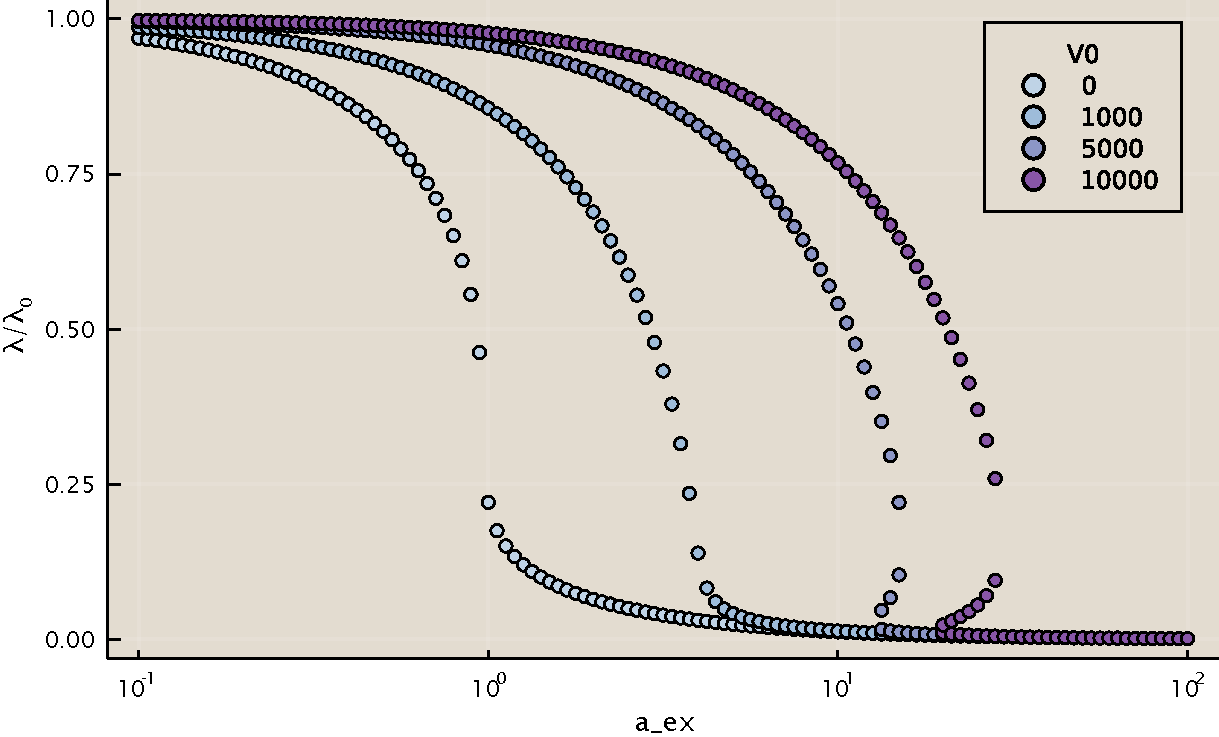
\includegraphics[width=.7\linewidth]{res_model_edit.pdf}
    \caption{Predicted relative growth rate $\lambda/\lambda_0$ at various levels of resistance $V_0$ for increasing extracellular drug concentration $a_\RM{ex}$.}
    \label{fig:model_res}
\end{figure}
\section{Statistical Mechanics of the Simple Repression Motif}
\label{sec:gene_expression}
